\subsection{Detecção de Bordas}

Em sistemas síncronos, as transições de estado ocorrem tipicamente nas bordas do sinal (subida ou descida), garantindo que todos os elementos de memória sejam atualizados de forma coordenada e evitando ambiguidades causadas por atrasos de propagação.

O detector de borda de subida identifica o momento em que um sinal transita de 0 para 1, gerando um pulso curto. Se este sinal for o clock ($clk$):

\begin{figure}[H]
    \centering
    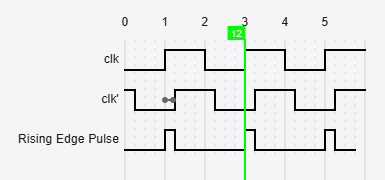
\includegraphics[width=0.7\linewidth]{images/rising-edge-detector-time-diagram.png}
    \caption{Timing digital do detector de borda de subida}
    \label{fig:rising-edge-detector-time-diagram}
\end{figure}

Esse comportamento pode ser descrito como:

\[
\text{Rising Edge} = clk \land \lnot clk_{delay}
\]

onde $clk_{delay}$ representa uma versão atrasada do sinal de clock, tal que $clk_{delay}(t) = clk(t - \Delta t)$.

Segue uma implementação do circuito de detecção de borda de subida: 

\begin{figure}[H]
    \centering
    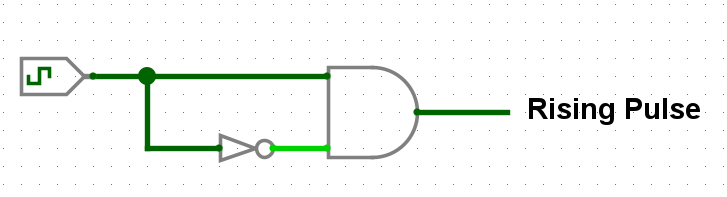
\includegraphics[width=0.7\linewidth]{images/rising-edge-detector.png}
    \caption{Detector de borda de subida}
    \label{fig:rising-edge-detector}
\end{figure}

O portão not introduz o delay $\Delta t$ ao mesmo tempo que respeita a equação acima.

\begin{figure}[H]
    \centering
    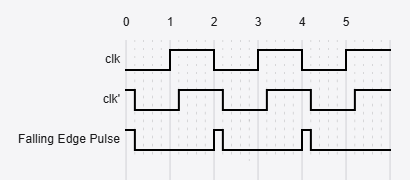
\includegraphics[width=0.7\linewidth]{images/falling-edge-detector-time-diagram.png}
    \caption{Timing digital do detector de borda de descida}
    \label{fig:falling-edge-detector-time-diagram}
\end{figure}

De forma análoga, o detector de borda de descida identifica a transição de 1 para 0:

\[
\text{Falling Edge} = \lnot clk \land clk_{delay}
\]

Uma implementação alternativa pode ser obtida a partir de uma transformação lógica utilizando as leis de De Morgan:

\[
\text{Falling Edge} = \lnot clk \land clk_{delay}
= \lnot (clk \lor \lnot clk_{delay})
\]

Essa forma é particularmente útil do ponto de vista de implementação, pois permite construir o detector utilizando uma porta NOR em conjunto com um inversor.

Nesse arranjo, o sinal $clk_{delay}$ é invertido e combinado com $clk$ por meio de uma porta NOR, produzindo diretamente o pulso correspondente à borda de descida.

Nesse caso, o pulso de saída é gerado no instante em que o sinal original já transitou para nível baixo, enquanto sua versão atrasada ainda permanece em nível alto, caracterizando a borda de descida.

\begin{figure}[H]
    \centering
    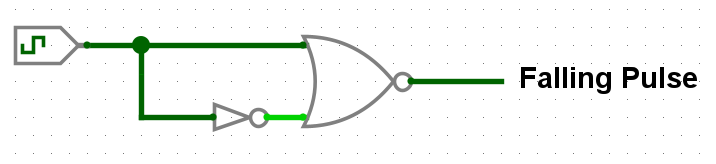
\includegraphics[width=0.7\linewidth]{images/falling-edge-detector.png}
    \caption{Detector de borda de descida}
    \label{fig:falling-edge-detector}
\end{figure}